
%----------------------------------------------------------------------------------------
%   Хавсралтууд эндээс эхэлнэ
%----------------------------------------------------------------------------------------
\appendix
\addcontentsline{toc}{part}{ХАВСРАЛТ}

% Хавсралтын нэр. Хавсралт гэдэг үг агуулахгүй
\section{Үечилсэн төлөвлөгөө}
\begin{figure}[h]
	\centering
	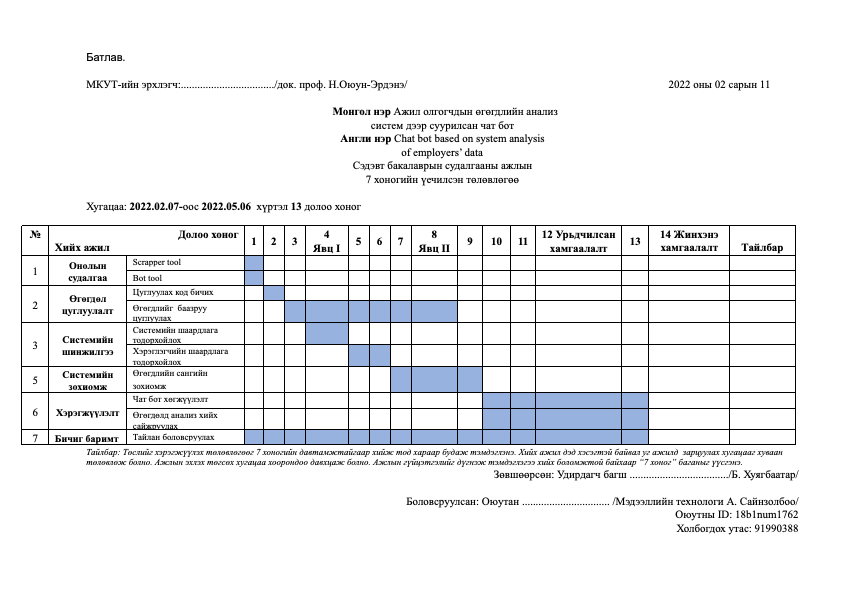
\includegraphics[width=16.5cm, angle=90]{images/plan.png}
	\caption{Бакалаврын судалгааны ажлын үечилсэн төлөвлөгөө}
	\label{fig:plan01}
	\end{figure}
% Хавсралтын нэр. Хавсралт гэдэг үг агуулахгүй
\chapter{Кодын хэрэгжүүлэлт}

\section{Өгөгдөл цугуулалт}
Beautiful Soup ашиглан үндсэн өгөгдлийг цуглуулах програм нь дараах бүтэцтэй байна.
\begin{itemize}
\end{itemize}
\subsection{Beautiful Soup ашиглан үндсэн өгөгдлийг цуглуулах эх код}
\lstinputlisting[language=Python, caption=xd]{code/dataScrapping.py}
% \begin{lstlisting}[language=Python]{../hello.c}